\chapter{Технологический раздел}

\section{Выбор средств разработки}

Для реализации метода поддержки принятия решений в рамках выполнения пошаговой инструкции, заданной в графовом формате, был выбран Python~\cite{python} по следующим причинам:
\begin{itemize}
    \item язык программирования позволяет быстро создавать рабочие прототипы в связи с наличием большого количества библиотек;
    \item имеются библиотеки для научных вычислений и визуализации (NumPy, Matplotlib, NetworkX);
    \item наличие опыта работы с языком программирования.
\end{itemize}

В качестве дополнительных библиотек были использованы следующие.

\begin{itemize}
    \item \textbf{NumPy}: для выполнения матричных операций при вычислении весов критериев. 
    Использование NumPy позволяет ускорить вычисления по сравнению с реализациями, написанными с помощью стандартной библиотеки Python.
    \item \textbf{NetworkX}: для построения ориентированного графа инструкций и его визуализации. 
    Библиотека предоставляет средства для работы с графами, включая алгоритмы поиска путей и компоновки узлов.
    \item \textbf{Matplotlib}: для отрисовки графа инструкций, размещения узлов и подписей, связей и легенды. 
\end{itemize}

В качестве среды разработки был выбран Visual Studio Code~\cite{vscode} по следующим причинам:
\begin{itemize}
    \item данный редактор позволяет удобно управлять всеми файлами проекта;
    \item наличие расширений, позволяющих работать с множеством форматов файлов и языков;
    \item наличие опыта работы с данном редактором.
\end{itemize}

Для хранения информации о графах, весах критериев и метках был выбран формат файлов JSON~\cite{json} по следующим причинам:
\begin{itemize}
    \item отсутствие привязки к конкретному языку программирования;
    \item простота чтения;
    \item частое использование на практике;
    \item широкая поддержка со стороны разработчиков.
\end{itemize}

\section{Реализация программного обеспечения}

\subsection{Разбиение на модули}

Программная система реализована в виде набора модулей, каждый из которых отвечает за определенную функциональность.

\begin{itemize}
    \item \texttt{models.py} --- содержит классы данных, описывающие предметную область: \texttt{StateType} (типы состояний), \texttt{Object} (объекты и субъекты), \texttt{State} (состояния), \texttt{Action} (действия), \texttt{Label} (метки), \texttt{HistoryStep} (шаги истории).

    \item \texttt{graph.py} --- класс \texttt{InstructionGraph}, реализующий загрузку графа из JSON, проверку переходов, выполнение действий, управление историей и вывод текстового представления графа.

    \item \texttt{labels.py} --- класс \texttt{LabelManager}, обеспечивающий загрузку меток из конфигурационного файла, сопоставление действий с метками по ключевым словам (с кэшированием) и предоставление рекомендаций через \texttt{AHPRecommendationRanker}.

    \item \texttt{ahp\_method.py} --- класс \texttt{AHPMethod} (реализация МАИ для критериев: матрица попарных сравнений, вычисление весов через геометрическое среднее, проверка согласованности) и класс \texttt{AHPRecommendationRanker} (ранжирование рекомендаций на основе весов критериев с последующей нормализацией).

    \item \texttt{visualization.py} --- функция \texttt{visualize\_graph}, строящая графическое представление графа инструкций с помощью Matplotlib и NetworkX.

    \item \texttt{emergency.py} --- класс \texttt{EmergencyHandler}, отвечающий за загрузку, фильтрацию (по пересечению меток с ключевыми словами меток действия) и выполнение аварийных сценариев с поддержкой рекурсии.

    \item \texttt{debug\_mode.py} --- класс \texttt{DebugMode}, предоставляющий интерфейс для экспертной настройки весов и оценок, а также логирование изменений.

    \item \texttt{ahp\_full.py} --- содержит два класса: \texttt{FullAHP} (классический МАИ с попарным сравнением всех альтернатив) и \texttt{HierarchicalAHP} (модифицированный МАИ с рекурсивным жадным отбором на основе группировки).

    \item \texttt{main.py} --- точка входа, организующая диалог с пользователем, выбор уровня экспертизы, загрузку графа и вызов соответствующих режимов.
\end{itemize}

\subsection{Реализация ключевых алгоритмов}

\subsubsection{Алгоритм выбора уровня экспертизы}

Данный алгоритм реализован в функции \texttt{change\_profile} модуля \texttt{main.py}, а также при начальной загрузке программы. 

Входные данные: выбор пользователя (1, 2 или 3) в интерактивном меню.

Выходные данные: объект \texttt{LabelManager} с загруженным профилем и пересчитанными весами критериев.

Исходный код функции \texttt{change\_profile} приведен в листинге~\ref{lst:change_profile}.

% \begin{lstlisting}[frame=single, language=Python, caption={Фрагмент функции смены уровня экспертизы}, label={lst:change_profile}]
%     def change_profile(label_manager, choice):
%         profile_map = {'1':'new', '2':'experienced', '3':'expert'}
%         new_profile = profile_map.get(choice, 'experienced')
%         labels_cfg = os.path.join(BASE_DIR, "labels_config.json")
%         ahp_cfg = os.path.join(BASE_DIR, "ahp_criteria_config.json")
%         new_lm = LabelManager(labels_cfg, ahp_cfg, profile=new_profile)
%         return new_lm
% \end{lstlisting}

\subsubsection{Функция загрузки графа инструкций}

Входные данные:
\begin{itemize}
    \item json\_file --- строка, путь к JSON-файлу, содержащему описание графа (состояния, действия, переходы, объекты);
    \item label\_manager --- объект класса \texttt{LabelManager}, используемый для сопоставления действий с метками.
\end{itemize}

Выходные данные: объект класса \texttt{InstructionGraph}, заполненный состояниями, действиями и переходами из JSON-файла.

Исходный код метода \texttt{from\_json} приведен в листинге~\ref{lst:loadgraph}.


% \begin{lstlisting}[frame=single, language=Python, caption={Загрузка графа из JSON}, label={lst:loadgraph}]
% def from_json(cls, json_file: str, label_manager=None):
%     with open(json_file, 'r', encoding='utf-8') as f:
%         data = json.load(f)
%     graph = cls(data.get('name', 'InstructionGraph'), label_manager)
%     for obj_data in data.get('objects', []):
%         graph.add_object(Object(
%             name=obj_data['name'],
%             obj_type=obj_data.get('type', 'object'),
%             properties={}
%         ))
%     for state_data in data.get('states', []):
%         graph.add_state(State(
%             id=state_data['id'],
%             name=state_data['name'],
%             description=state_data.get('description', ''),
%             state_type=StateType.from_string(state_data.get('type', 'intermediate')),
%             objects_state=state_data.get('objects_state', {})
%         ))
%     for action_data in data.get('actions', []):
%         graph.add_action(Action(
%             id=action_data['id'],
%             name=action_data['name'],
%             description=action_data.get('description', ''),
%             required_objects=set(action_data.get('required_objects', []))
%         ))
%     for trans_data in data.get('transitions', []):
%         graph.add_transition(trans_data['from'], trans_data['action'], trans_data['to'])
%     return graph
% \end{lstlisting}

\subsubsection{Функция выполнения действия в пошаговом режиме}

Входные данные:
\begin{itemize}
    \item action\_id --- строка, идентификатор действия, выбранного пользователем;
    \item recommendations --- список словарей, содержащих рекомендации, показанные пользователю (каждый словарь имеет поля \texttt{text} и \texttt{score});
    \item silent --- булевый флаг, подавляющий вывод сообщений.
\end{itemize}

Выходные данные: булево значение \texttt{True}, если действие успешно выполнено (переход в новое состояние), иначе \texttt{False}.

В листинге~\ref{lst:execute} приведен метод \texttt{execute\_action} класса \texttt{InstructionGraph}.

% \begin{lstlisting}[frame=single, language=Python, caption={Выполнение действия}, label={lst:execute}]
% def execute_action(self, action_id: str, recommendations=None, silent=False):
%     if self.current_state_id is None:
%         return False
%     transition_key = (self.current_state_id, action_id)
%     if transition_key not in self.transitions:
%         return False
%     next_state_id = self.transitions[transition_key]
%     old_state = self.current_state_id
%     old_state_name = self.states[old_state].name
%     self.current_state_id = next_state_id
%     new_state_name = self.states[self.current_state_id].name
%     history_step = HistoryStep(
%         from_state=old_state,
%         from_state_name=old_state_name,
%         action_id=action_id,
%         action_name=self.actions[action_id].name,
%         to_state=self.current_state_id,
%         to_state_name=new_state_name,
%         recommendations=recommendations or []
%     )
%     self.execution_history.append(history_step)
%     return True
% \end{lstlisting}

\subsubsection{Функция ранжирования рекомендаций}

Входные данные:
\begin{itemize}
    \item recommendations --- список словарей, каждый из которых содержит поле \texttt{scores} (оценки по критериям) и \texttt{text};
    \item top\_n --- целое число, обозначает количество лучших рекомендаций, которое требуется вернуть.
\end{itemize}

Выходные данные: список словарей, каждый из которых содержит поля \texttt{text} (текст рекомендации), \texttt{score} (нормализованная интегральная оценка) и \texttt{rank} (порядковый номер).

Исходный код метода \texttt{rank\_recommendations} класса \texttt{AHPRecommendationRanker} приведен в листинге~\ref{lst:rank}.

% \begin{lstlisting}[frame=single, language=Python,caption={Ранжирование рекомендаций}, label={lst:rank}]
% def rank_recommendations(self, recommendations, top_n=3):
%     raw_scores = [self.calculate_recommendation_score(rec.get('scores', {})) for rec in recommendations]
%     total = sum(raw_scores)
%     if total > 0:
%         norm_scores = [s / total for s in raw_scores]
%     else:
%         norm_scores = [1.0 / len(recommendations)] * len(recommendations)
%     ranked = sorted(zip(recommendations, norm_scores), key=lambda x: x[1], reverse=True)
%     return [{'text': rec['text'], 'score': score, 'rank': i+1} for i, (rec, score) in enumerate(ranked[:top_n])]
% \end{lstlisting}

\clearpage
\subsubsection{Функция запуска аварийного сценария}

Входные данные:
\begin{itemize}
    \item scenario\_id --- строка, идентификатор аварийного сценария (например, \texttt{spilled\_water});
    \item recursion\_depth --- целое число (по умолчанию 0), текущая глубина вложенности аварийного сценария.
\end{itemize}

Выходные данные: булево значение \texttt{return\_to\_original}, указывающее, нужно ли вернуться к основному графу после завершения сценария.

Реализация метода \texttt{run\_emergency\_scenario} класса \texttt{EmergencyHandler} представлена в листинге~\ref{lst:emergency}.

% \begin{lstlisting}[frame=single, language=Python, caption={Выполнение аварийного сценария}, label={lst:emergency}]
% def run_emergency_scenario(self, scenario_id, recursion_depth=0):
%     if recursion_depth >= self.max_depth:
%         return True
%     graph = self.load_emergency_graph(scenario_id)
%     if not graph:
%         return True
%     info = self.scenarios_config[scenario_id]
%     self._run_emergency_steps(graph, recursion_depth + 1)
%     return info.get('return_to_original', True)
% \end{lstlisting}

\subsubsection{Реализация модифицированного метода МАИ}

Входные данные:
\begin{itemize}
    \item element --- строка, имя текущего элемента (группы или альтернативы);
    \item limit --- целое число, максимальное количество листьев, которое требуется собрать;
    \item depth --- целое число, текущая глубина рекурсии.
\end{itemize}

Выходные данные: список словарей, каждый из которых содержит поле \texttt{alternative}.

Исходный код метода \texttt{\_collect\_leaves} класса \texttt{HierarchicalAHP} приведен в листинге~\ref{lst:collect}.

% \begin{lstlisting}[frame=single, language=Python,caption={Рекурсивный сбор лучших рекомендаций в групповом МАИ}, label={lst:collect}]
% def _collect_leaves(self, element: str, limit: int, depth: int = 0):
%     if element not in self.elements_data:
%         return [{'alternative': element, 'priority': 1.0}]
%     children = self.elements_data[element]
%     if not children:
%         return []
%     aggregated = self._get_aggregated_weights(element, children)
%     sorted_children = sorted(aggregated.items(), key=lambda x: x[1], reverse=True)
%     result = []
%     for child, _ in sorted_children:
%         if len(result) >= limit:
%             break
%         result.extend(self._collect_leaves(child, limit - len(result), depth + 1))
%     return result
% \end{lstlisting}

\subsection{Формат используемых файлов}

\subsubsection{Файл графа инструкции}

На рисунке~\ref{fig:graph} представлен пример файла графового описания инструкции.

\begin{figure}[H]
	\centering
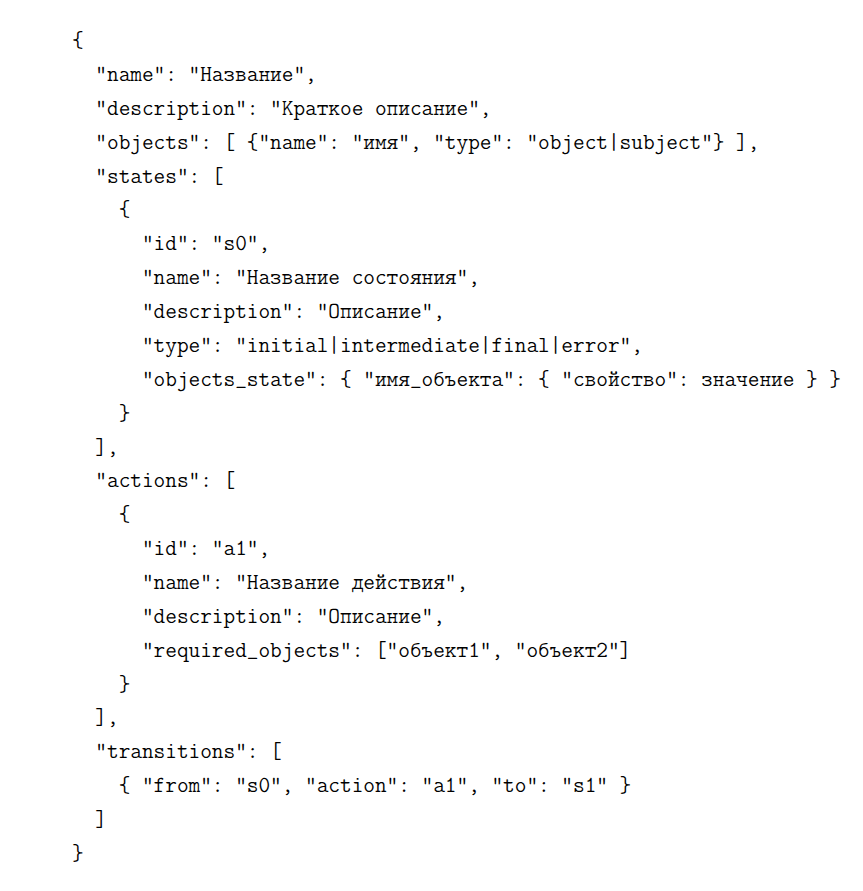
\includegraphics[width=0.9\linewidth]{inc/img/json1.png}
	\caption{Пример файла графового описания инструкции}
	\label{fig:graph}
\end{figure}

Поля \texttt{objects\_state} описывают свойства объектов в каждом состоянии.
Значения свойств могут быть булевыми, числами или строками.

\subsubsection{Файл меток и рекомендаций}

Файл \texttt{labels\_config.json} содержит массив меток, каждая из которых имеет имя, список ключевых слов и массив рекомендаций.
Каждая рекомендация содержит текст и оценки по каждому критерию в виде словаря \texttt{scores}.

Пример фрагмента файла представлен на рисунке~\ref{fig:marks}.

\begin{figure}[H]
	\centering
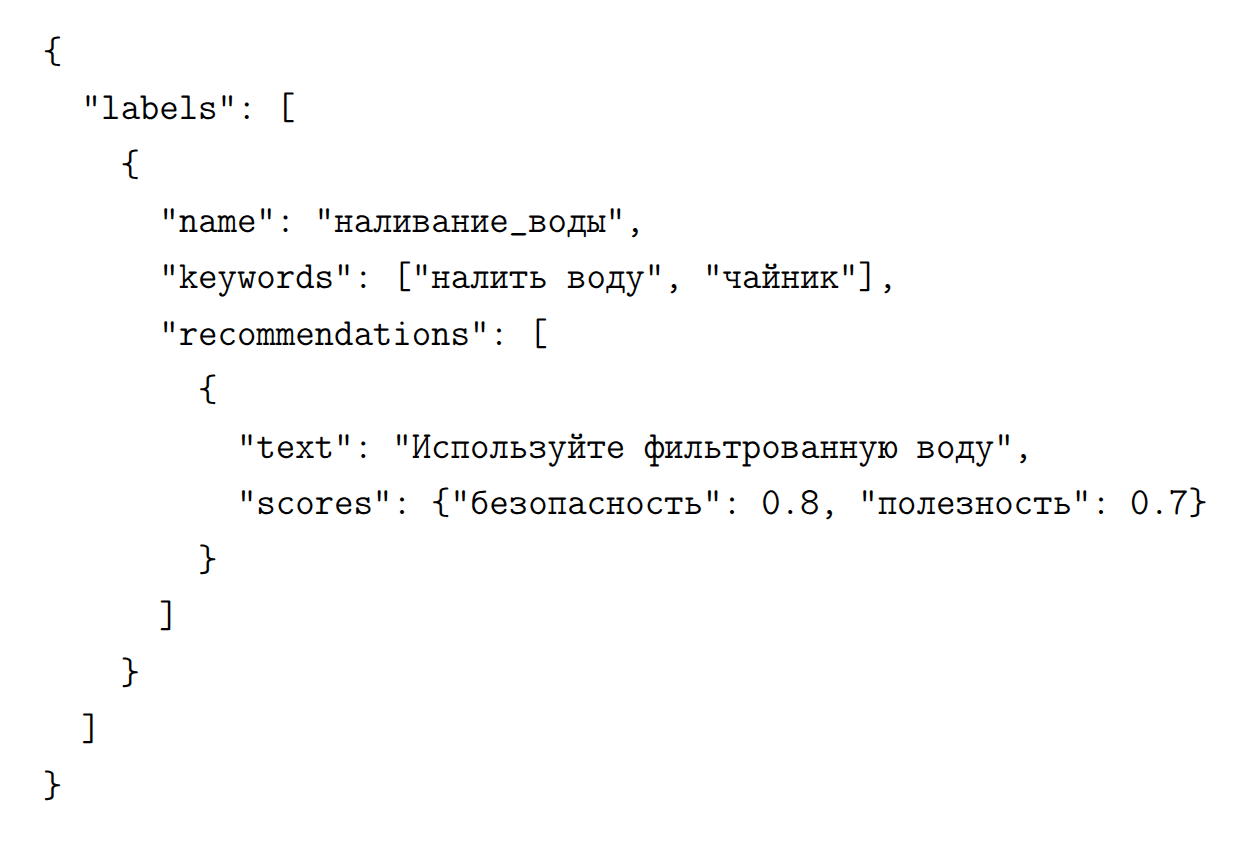
\includegraphics[width=0.9\linewidth]{inc/img/json2.png}
	\caption{Пример фрагмента файла меток}
	\label{fig:marks}
\end{figure}

\subsubsection{Файл критериев МАИ с профилями экспертизы}

Файл \texttt{ahp\_criteria\_config.json} содержит список критериев и три профиля (новичок, опытный, эксперт). 
Для каждого профиля задаются попарные сравнения критериев в виде словаря \texttt{pairwise\_comparisons}, где ключи имеют вид \texttt{критерий1\_vs\_критерий2}. 
Значения --- числа от 1 до 9 (и обратные им от 1 до 1/9).
Допускается также поле \texttt{calculated\_weights} для прямого задания весов (используется при генерации из режима отладки).

\subsubsection{Файл конфигурации аварийных сценариев}

Файл \texttt{emergency\_scenarios.json} является словарем, где именем является название аварийного сценария, в нем содержится имя файла, в котором хранится аварийный сценарий, его описание, флаг возможности возврата и соответствующие сценарию метки.

Пример фрагмента файла представлен на рисунке \ref{figs:emergency}.

\begin{figure}[H]
	\centering
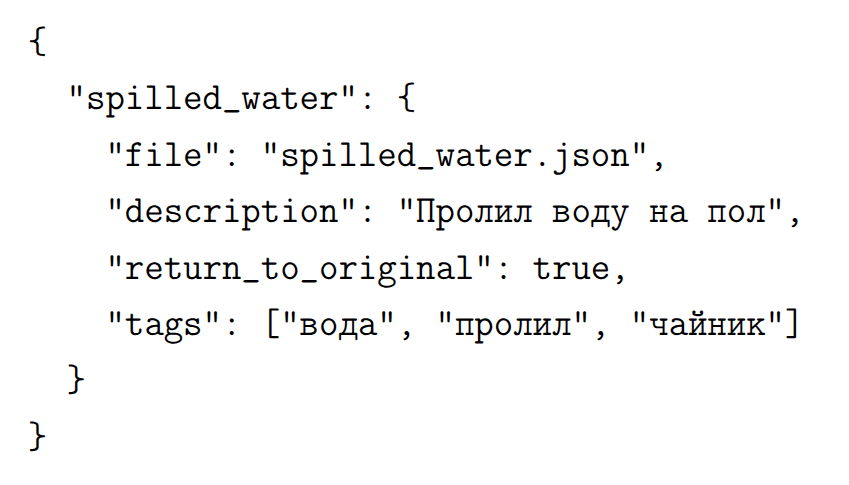
\includegraphics[width=0.6\linewidth]{inc/img/json3.png}
	\caption{Пример фрагмента файла аварийного сценария}
	\label{figs:emergency}
\end{figure}

\section{Описание взаимодействия пользователя с программой}

\subsection*{Выбор уровня экспертизы}

После запуска пользователю предлагается выбрать один из трех уровней экспертизы.

\begin{enumerate}
    \item \textbf{Новичок} --- максимальный приоритет безопасности.
    \item \textbf{Опытный} --- сбалансированные веса.
    \item \textbf{Эксперт} --- приоритет критичности и полезности.
\end{enumerate}

Выбор уровня влияет на веса критериев, используемые при ранжировании рекомендаций.

\subsection*{Главное меню}

После загрузки графа отображается главное меню, представленное на рисунке~\ref{fig:menu}.
\begin{figure}[H]
	\centering

\includegraphics[width=0.8\linewidth]{inc/img/menu.png}
	\caption{Главное меню программы}
	\label{fig:menu}
\end{figure}


Описание пунктов меню представлено далее.

\textbf{1. Пошаговый режим} --- запуск режима интерактивного пошагового выполнения инструкции.

\textbf{2. Вывести информацию о графе} --- вывод статистики (количество состояний, действий, объектов, переходов) и текущего состояния графа.

\textbf{3. Визуализация} --- построение графического изображения графа (сохраняется в PNG-файл и отображается на экране).

\textbf{4. Все метки} --- вывод всех загруженных меток с их ключевыми словами и рекомендациями.

\textbf{5. Вывести веса критериев} --- отображение текущих весов критериев, вычисленных методом МАИ, а также отношения согласованности (CR).

\textbf{6. Режим дебага} --- вход в режим экспертной отладки.

\textbf{7. Загрузить другой граф} --- позволяет выбрать новый JSON-файл инструкции без перезапуска программы.

\textbf{8. Сбросить состояние} --- возвращает граф в начальное состояние (очищает историю и сбрасывает текущее состояние).

\textbf{9. Сменить уровень экспертизы} --- изменить текущий профиль (пересчитать веса критериев).

\textbf{10. Сравнение реализованных методов МАИ} --- запуск сравнительного анализа классического МАИ и модифицированного МАИ. 

\textbf{0. Выход} --- завершение работы программы.

\subsection*{Пошаговый режим}

При выборе пункта 1 запускается интерактивное выполнение инструкции. 
На каждом шаге отображается следующая информация:
\begin{itemize}
\item текущее состояние графа;
\item состояние объектов;
\item список доступных действий с номерами и следующими состояниями;
\item для каждого действия --- перечень меток, которые к нему относится.
\end{itemize}

Пользователь может ввести номер действия для его выполнения, либо команду:

\begin{itemize}
\item \texttt{0} --- завершить пошаговый режим и сохранить результаты;
\item \texttt{i} --- показать подробную информацию о действии (описание, требуемые объекты, $5$ лучших рекомендаций);
\item \texttt{a} --- показать текущие веса критериев;
\item \texttt{q} --- показать историю выполненных шагов.
\end{itemize}

При выборе действия система выводит 3 лучшие рекомендации (текст и нормализованную оценку) и запрашивает подтверждение корректности выполненного действия.
Если пользователь отвечает <<Да>>, действие выполняется, и происходит переход в следующее состояние.
Если пользователь отвечает <<Нет>>, система спрашивает, возникла ли аварийная ситуация.
При утвердительном ответе предлагается список контекстно-зависимых аварийных сценариев, из которых пользователь может выбрать один.
Затем загружается и выполняется аварийный граф, после чего, в зависимости от флага сценария, происходит либо возврат к основному графу, либо выход в главное меню.

\clearpage
\subsection*{Режим отладки}

Пункт 6 главного меню открывает режим отладки для эксперта, в котором доступны следующие действия:

\begin{itemize}
\item просмотр текущих весов критериев;
\item изменение весов через ввод парных сравнений (по шкале Саати);
\item просмотр всех действий и их рекомендаций с оценками;
\item изменение оценок рекомендаций по каждому критерию;
\item пошаговое выполнение с отладочной информацией (вывод весов, вклада каждого критерия, детализированных оценок рекомендаций);
\item история изменений;
\item сохранение изменений в новые файлы (в директорию \texttt{debug}) с привязкой к текущему профилю;
\item сброс к оригинальным настройкам.
\end{itemize}

Изменения в режиме отладки не влияют на исходные конфигурационные файлы и сохраняются отдельно.

\subsection*{Визуализация графа}

Пункт 3 вызывает функцию \texttt{visualize\_graph}, которая строит графическое представление графа с помощью Matplotlib и NetworkX.
Состояния располагаются в центре, действия --- слева, объекты и субъекты --- справа.

\subsection*{Сравнение методов МАИ на примере заданного файла}

Пункт 10 главного меню позволяет провести сравнительный анализ двух реализаций метода анализа иерархий: классического и модифицированного.

При выборе этого пункта программа предлагает пользователю выбрать JSON-файл из директории \texttt{research/} для сравнения.

\clearpage
Файл должен содержать следующую информацию:
\begin{itemize}
\item список критериев и их попарные сравнения;
\item для классического метода --- поле \texttt{alternatives} (список всех альтернатив) и \texttt{comparisons\_by\_criterion} (попарные сравнения альтернатив по каждому критерию);
\item для модифицированного метода --- поле \texttt{hierarchy} (иерархия групп), \texttt{elements\_data} (состав групп) и \texttt{comparisons} (парные сравнения для каждого элемента).
\end{itemize}

После выбора файла программа последовательно выполняет оба метода и выводит результаты.

\begin{enumerate}
\item \textbf{Классический МАИ}:
\begin{itemize}
\item количество выполненных попарных сравнений (сумма сравнений критериев и всех альтернатив по каждому критерию);
\item 5 лучших альтернатив с их глобальными приоритетами.
\end{itemize}
\item \textbf{Модифицированный МАИ}:
\begin{itemize}
\item количество выполненных попарных сравнений (сумма сравнений критериев, сравнений групп и сравнений внутри групп);
\item количество групп в иерархии;
\item 5 лучших альтернатив (порядок определяется жадным рекурсивным обходом).
\end{itemize}
\end{enumerate}

Этот режим позволяет сравнить следующее:
\begin{itemize}
\item объем экспертной работы (количество попарных сравнений), требуемый для каждого метода;
\item различия в ранжировании альтернатив, вызванные группировкой;
\item эффективность модификации при большом количестве альтернатив.
\end{itemize}

Результаты сравнения могут быть сохранены в файлы в директории \texttt{debug/} для последующего анализа.

\subsection*{Сохранение результатов}

После завершения пошагового режима (или принудительного выхода) программа автоматически сохраняет файл \texttt{<имя\_графа>\_result.json} в директорию \texttt{result/}. 
Файл содержит следующую информацию:
\begin{itemize}
\item \texttt{execution\_history} --- массив шагов с указанием исходного и конечного состояний, выполненного действия и показанных рекомендаций;
\item \texttt{total\_steps} --- общее количество выполненных действий;
\item \texttt{final\_state\_id} --- идентификатор конечного состояния;
\item \texttt{final\_state\_name} --- идентификатор конечного состояния;
\item \texttt{final\_objects\_state} --- состояние всех объектов в конечном состоянии.
\end{itemize}

\section{Тестирование программного обеспечения}

Все функциональные тесты, описанные в таблицах~\ref{tab:tests1},~\ref{tab:tests2},~\ref{tab:tests3}, пройдены успешно.

\phantomsection
\section*{Выводы}
\addcontentsline{toc}{section}{Выводы}


В данном разделе был обоснован выбор средств разработки.
Описана структура ПО, форматы входных и выходных файлов.
Описаны выполненные реализации ключевых алгоритмов.
Представлены результаты тестирования, подтверждающие корректность работы всех компонентов.